\documentclass[a4paper, 12pt]{article}
\usepackage[top=2cm, bottom=2cm, left=2.5cm, right=2.5cm]{geometry}
\usepackage[utf8]{inputenc}
\usepackage[brazilian]{babel}
\usepackage{indentfirst}
\usepackage{graphicx}
\usepackage{wrapfig}
\usepackage[pdftex]{hyperref}
\graphicspath{ {imagens/} }
\usepackage{amsmath}

\begin{document}
%
\begin{titlepage} %iniciando a "capa"
	\begin{center} %centralizar o texto abaixo
		{\large Unicamp}\\[0.4cm] %0,2cm é a distância entre o texto dessa linha e o texto da próxima
		{\large Marco Lucio Bittencourt - Turma B}\\
		{\large Heitor Nigro Lopes - PED}\\[3.2cm]
		{\bf \huge Dinâmica Trabalho 2}\\[0.2cm] 
		{\bf \large Matrizes de Rotação e Range Kutta}\\[4.9cm]
		% o comando \bf deixa o texto entre chaves em negrito. O comando \huge deixa o texto enorme
	\end{center} %término do comando centralizar
	{\large Erik Yuji Goto}\\ % o comando \large deixa o texto grande
	RA: 234009\\[10cm]
	\begin{center}
	
		{\large Campinas}\\[0.2cm]
		{\large 2021}
	\end{center}
\end{titlepage} %término da "capa"


\tableofcontents
\newpage

\section{Observação}
	Não está englobado o material da P1
	\newpage
\section{Fasores}
	\begin{itemize}
		\item Resistor:\begin{equation}
			\underline{V_R} = R\underline{I_R}
		\end{equation}
		\item Indutor:\begin{equation}
			\underline{V_L} = j\omega L\underline{I_L}
		\end{equation}
		\item Capacitor:\begin{equation}
			\underline{V_C} = \frac{1}{j\omega C} \underline{I_C}
		\end{equation}
	\end{itemize}
	
\section{Impedância e Admitância}
	Define-se a impedância(Z) como a relação da tensão fasorial pela corrente fasorial:
	\begin{equation}
		Z = \frac{V_m}{I_m} \angle (\theta - \phi) = R + jX
	\end{equation}
	R é a componente resistivam e X é a componente reativa.\\
	A a admitância Y é o inverso da impedância.
	
	\begin{figure}[h]
		\centering
		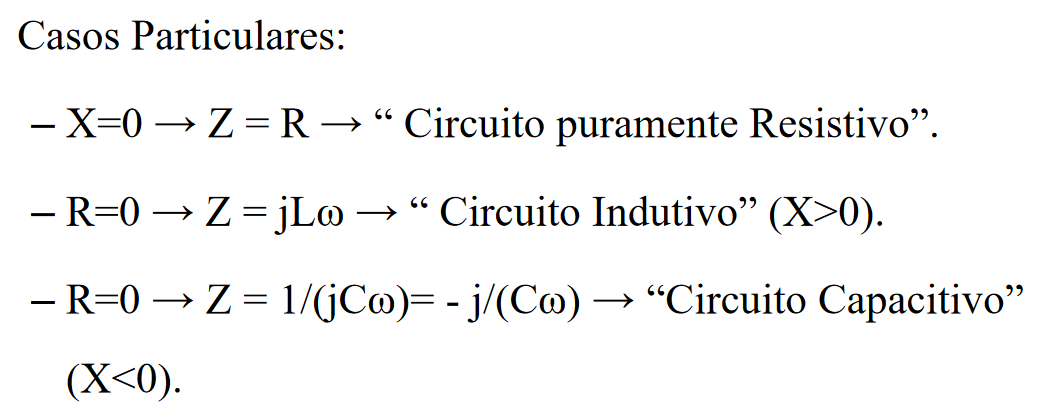
\includegraphics[scale=0.3]{a.png}
		\caption{Casos Particulares}
	\end{figure}
	
	\subsection{Associação de Impedâncias}
		\subsubsection{Série}
		\begin{equation}
			Z_{eq} = Z_1 + Z_2 + ... + Z_k 
		\end{equation}
		\subsubsection{Paralelo}
		\begin{equation}
			\frac{1}{Z_{eq}} = \frac{1}{Z_1} + \frac{1}{Z_2} + ... + \frac{1}{Z_k}
		\end{equation}
	
\section{Potência em excitações senoidais}
	\subsection{Potência Média}
		\begin{equation}
			\bar{p} = \frac{V_mI_m}{2} cos\theta
		\end{equation}
	
	\subsection{Valores Eficazes}
		O valor eficaz de uma corrente(tensão) periódica é equivalente a uma corrente(tensão) contínua que entrega a mesma potência média para um resistor:
		\begin{equation}
			I_{ef} = \frac{I_m}{\sqrt{2}}
		\end{equation}
		\begin{equation}
			V_{ef} = \frac{V_m}{\sqrt{2}}
		\end{equation}
		Portanto, a potência média fica:
		\begin{equation}
			\bar{p} = I_{ef} V_{ef} cos \theta
		\end{equation}
		Onde o produto $I_{ef}*V_{ef}$ é definido como a potência aparente.
		
	\subsection{Fator de Potência}
		O fator de potência ($f_p$) é definido como a relação entre a
potência média e a potência aparente:
		\begin{equation}
			f_p = cos\theta
		\end{equation}

		\begin{itemize}
			\item Carga RC - fator de potência adiantado;
			\item Carga RL - fator de potência atrasado;
		\end{itemize}
		Na prática é comum acrescentar um elemento puramente reativo (resistência nula) em paralelo com a impedância original, de modo a alterar o fator de potência ao nível desejado.

	\subsubsection{Correção do fator de Potência}
		Seja um sistema elétrico representado por uma impedância $Z= R + j X$. Suponha que em paralelo a esta
impedância é acrescentado o elemento $Z1= jX1$. Então, podemos calcular o valor da impedância em paralelo:
		\begin{equation}
			X_1 = \frac{R^2 + X^2}{R.tg(cos^{-1} f_p) - X}
		\end{equation}
		
	\newpage
	\subsection{Potência Complexa}
		A potência complexa é definida por:
		\begin{equation}
			S = \underline{V}_{ef}\underline{I}_{ef}^* = P + jQ
		\end{equation}
		$\underline{I}_{ef}^*$ é o conjugado da corrente eficaz.\\
		P é a potência ativa e Q a potência reativa.
		\begin{figure}[h]
			\centering
			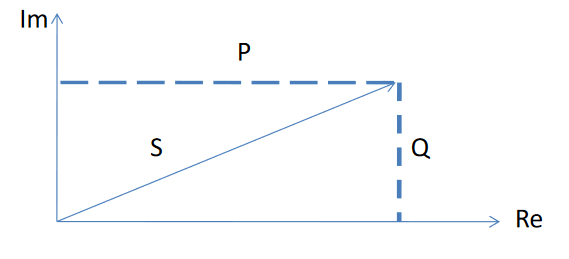
\includegraphics[scale=0.5]{a1.png}
			\caption{Potência Complexa}
		\end{figure}\\
		O módulo da potência complexa é dado por:
			\begin{equation}
				|S| = V_{ef}I_{ef}
			\end{equation}
		Que é igual à potência aparente. Então, a potência reativa Q é dada por:
			\begin{equation}
				Q = Im (S) = V_{ef}I_{ef}sin\theta
			\end{equation}
		Lembre que, a carga atendida é dada por:
			\begin{equation}
				Z = R + jX
			\end{equation}
	
	\subsection{Correção de $f_p$ em termos de potência}
		Uma potência complexa S é fornecido à carga Z. A potência fornecida pode ser decomposta em:
			\begin{equation}
				S = P + jQ
			\end{equation}
			Acrescenta-se uma carga de reatância pura Z1 em paralelo com Z. Com isso a potência complexa total fornecida ao circuito será:
			\begin{equation}
				S_T = P + j(Q + Q_1)
			\end{equation}

\section{Sistemas Trifásicos}
	Os sistemas trifásicos são constituídos de três sistemas monofásicos defasadas de 120. Usualmente as fases são nomeadas em a,b e c:
	\begin{figure}[h]
		\centering
		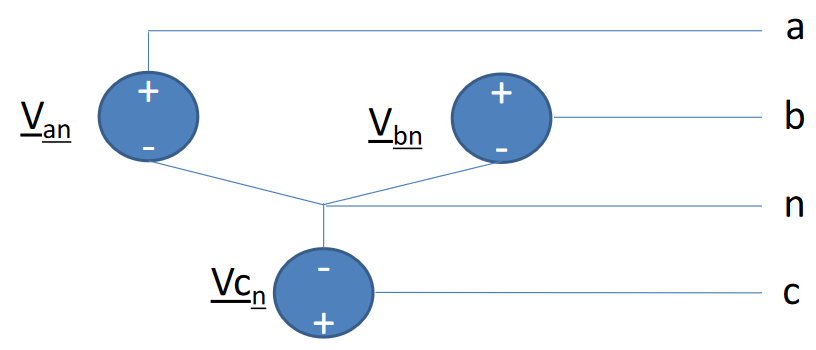
\includegraphics[scale=0.5]{a2.png}
		\caption{Sistema Trifásico}
	\end{figure}

	\begin{equation}
		v_a = V_p cos(\omega t) 
	\end{equation}
	\begin{equation}
		v_b = V_p cos(\omega t - 120)
	\end{equation}
	\begin{equation}
		v_c = V_p cos(\omega t + 120)
	\end{equation}

	\textbf{Tensão de Fase} é a tenão nos terminais das fontes trifásicas.
	\begin{equation}
		\underline{V_{an}} = V_p \angle 0
	\end{equation}
	\begin{equation}
		\underline{V_{bn}} = V_p \angle -120
	\end{equation}
	\begin{equation}
		\underline{V_{cn}} = V_p \angle 120
	\end{equation}

	\textbf{Tensão entre fases} é dado pela diferença de tensões de fase.
	\begin{equation}
		\underline{V_{ab}} = \sqrt{3}V_p \angle 30
	\end{equation}
	É importante destacar que no caso da tensão fasorial $\underline{V_{ab}}$ a
fase “a” é a referência. Com isso a fase do fasor da tensão entre as fases “a” e “b” é de 30º em relação à fase a.	
	
	De forma similar temos:
		\begin{equation}
			\underline{V_{bc}} = \sqrt{3}V_p \angle -90
		\end{equation}
		\begin{equation}
			\underline{V_{ca}} = \sqrt{3}V_p \angle 150
		\end{equation}

	\textbf{Convenção:}
	\begin{itemize}
		\item Os dados e variáveis relativos às conexões entre fontes e cargas são de linhas. Por exemplo, a corrente na conexão entre uma fonte e uma carga é dita corrente de linha;
		\item Os dados e variáveis relativos às fontes e cargas são de fase. Por exemplo, a tensão em uma carga é denominada tensão de fase.
	\end{itemize}

\newpage
\section{Conexão em Y-Y}
	\begin{figure}[h]
		\centering
		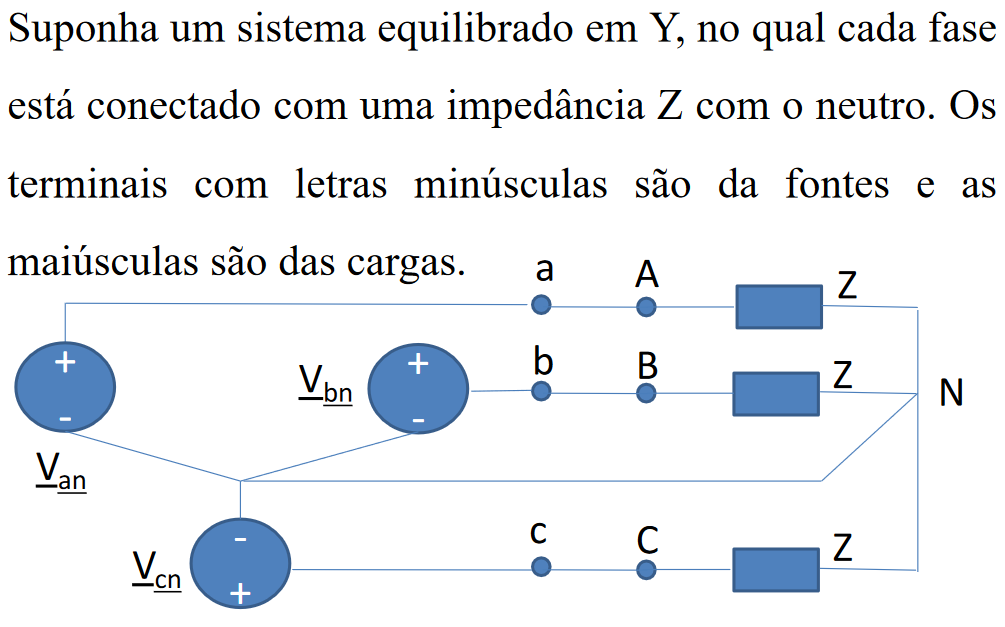
\includegraphics[scale=0.3]{a3.png}
		\caption{Conexão em Y-Y}
	\end{figure}
	Neste caso a impedância Z da fase A está conectada entre a saída da fonte a e o neutro. Então, a corrente sobre esta impedância é dada por:
	\begin{equation}
		\underline{I_{aA}} = \frac{\underline{V_{an}}}{Z} = I_{aA}\angle - \theta
	\end{equation}

	As correntes das outras cargas tem a mesma amplitude e com as fases defasadas de -120 e +120.
	\begin{equation}
		\underline{I_{bB}} = I_{aA} \angle (-120 - \theta)
	\end{equation}
	\begin{equation}
		\underline{I_{cC}} = I_{aA} \angle (120-\theta)
	\end{equation}

	Note que, numa conexão Y-Y equilibrada a quatro fios, a soma das três correntes de linha é nula. Portanto, a corrente pelo neutro é nula.\\
	
	A potência média entregur pela fase p é:
	\begin{equation}
		P_p = V_pI_p cos\theta
	\end{equation}
	Então a potência total entregue pelas 3 fases é:
	\begin{equation}
		P = 3P
	\end{equation}
	
\section{Conexão em Delta}
	\begin{figure}[h]
		\centering
		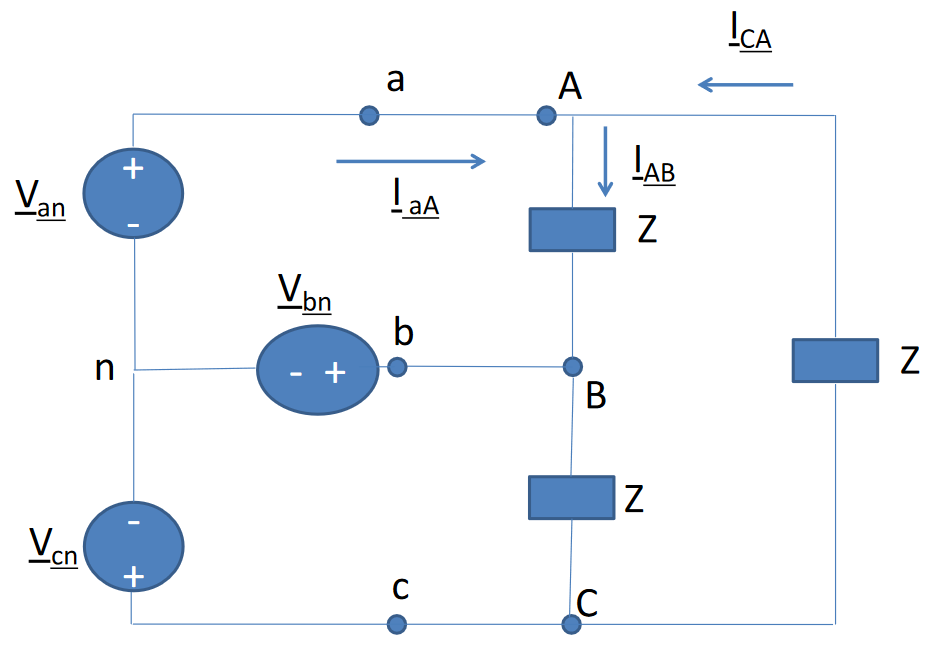
\includegraphics[scale=0.4]{a4.png}
		\caption{Conexão em Delta}
	\end{figure}
	\newpage
	Nesta configuração as impedâncias estão conectadas entre duas fases e não com o neutro.
	
	Já foi visto que as tensões entre fases são dadas por:
	\begin{equation}
		\underline{V_{AB}} = V_L \angle 30
	\end{equation}
	\begin{equation}
		\underline{V_{BC}} = V_L \angle -90
	\end{equation}
	\begin{equation}
		\underline{V_{CA}} = V_L \angle 150
	\end{equation}
	
	Onde,\\
	$V_L = \sqrt{3}V_p$\\
	
	As correntes de fase são dadas por:
	\begin{equation}
		\underline{I_{AB}} =  \frac{V_L \angle 30}{|Z| \angle \theta} = I_Z \angle(30 - \theta)
	\end{equation}
	\begin{equation}
		\underline{I_{BC}} =  \frac{V_L \angle -90}{|Z| \angle \theta} = I_Z \angle(-90 - \theta)
	\end{equation}
	\begin{equation}
		\underline{I_{CA}} =  \frac{V_L \angle 150}{|Z| \angle \theta} = I_Z \angle(150 - \theta)
	\end{equation}

	Por sua vez, a amplitude da corrente de linha é igual à corrente de fase multiplicada por $\sqrt{3}$. E a fase da corrente de linha é igual à fase da corrente na carga subtraída de 30º.
	\begin{equation}
		\underline{I_{aA}} = \sqrt{3}I_Z \angle -\theta
	\end{equation}
	\begin{equation}
		\underline{I_{bB}} = \sqrt{3}I_Z \angle (-120-\theta)
	\end{equation}
	\begin{equation}
		\underline{I_{cC}} = \sqrt{3}I_Z \angle (120-\theta)
	\end{equation}

\section{Transformação Y - $\Delta$}
	É possível transformar uma conexão de cargas equilibradas em Y em uma configuração equivalente em $\Delta$, ou vice-versa

	\subsection{Transformação de Y para $\Delta$}
		\begin{figure}[h]
			\centering
			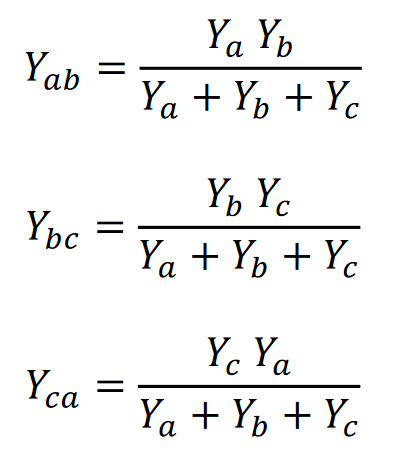
\includegraphics[scale=0.4]{a5.png}
			\caption{Transformação de Y para $\Delta$}
		\end{figure}
	\subsection{Transformação de $\Delta$ para Y}
		\begin{figure}[h]
			\centering
			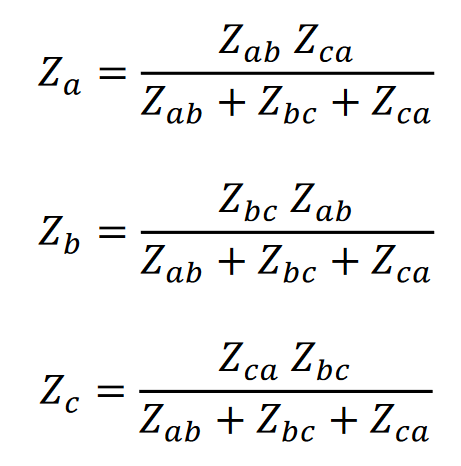
\includegraphics[scale=0.4]{a6.png}
			\caption{Transformação de $\Delta$ para Y}
		\end{figure}


















\end{document}
